\subsection{Influence of wrong assumptions about incompleteness of the data parallel to the Galactic plane} \label{sec:incompZ}

In \S\ref{sec:results_incompR} we found a striking robustness of the \RM modelling approach against wrong assumptions about the radial incompleteness of the data set. To further test this result, we investigate a different completeness function that drops with distance from the Galactic plane (see Test \ref{test:isoSphFlexIncomp}, Example 2, in Table \ref{tbl:tests} and Figure \ref{fig:isoSphFlexIncompZ_mockdata}). We get a similar robust behaviour for small deviations, and only slightly less robustness for larger deviations. That an explanation for this robustness could be, that much of the information about the potential comes from the rotation curve, which is not affected by incompleteness, is demonstrated in Figure \ref{fig:isoSphFlexIncomp_marginal_violins}.

\paragraph{Marginalization over $v_T$.} The likelihood in Equation \ref{eq:prob} is marginalized over the coordinate $v_T$ as follows
\begin{eqnarray*}
&&\left. \mathscr{L}(\pmodel \mid D)\right|_\text{($v_T$ marg.)}\\
&=& \prod_i^N P_\text{($v_T$ marg.)} (\vect{x}_i,v_{R,i},v_{z,i} \mid \pmodel)\\
&\equiv& \prod_i^N v_0 \cdot \int_0^{1.5v_\text{circ}(R_\odot)} \diff v_T \ P(\vect{x}_i,v_{R,i},v_{T},v_{z,i} \mid \pmodel )
\end{eqnarray*}
where $P(\vect{x},\vect{v} \mid \pmodel)$ is the same as in Equation \ref{eq:prob} and the numerical integral over $v_T$ is performed as a 24th order Gauss-Legendre quadrature. The additional factor of $v_0$ is needed to get the units of $P_\text{($v_T$ marg.)} (\vect{x}_i,v_{R,i},v_{z,i} \mid \pmodel)$ right.

%FIGURE:  isoSphFlexIncompZ
\begin{figure}
\centering
\begin{minipage}{.45\textwidth}
  \centering
\includegraphics[width=0.8\textwidth]{figs/isoSphFlexIncompZ_mockdata.eps}
\caption{Selection function and mock data distribution for investigating vertical incompleteness of the data. All model parameters are summarized as Test \ref{test:isoSphFlexIncomp}, Example 2, in Table \ref{tbl:tests}. The survey volume is a sphere around the sun and the percentage of observed stars is decreasing linearly with distance from the Galactic plane, as demonstrated in the left panel. How fast this detection/incompleteness rate drops is quantized by the factor $\epsilon_z$. Histograms for four data sets, drawn from two \MAPs{} (\texttt{hot} in red and \texttt{cool} in blue, see Table \ref{tbl:referenceMAPs}) and with two different $\epsilon_z$, 0 and 0.7, are shown in the right panel for illustration purposes. \Wilma{[TO DO: Potential and/or population names in typewriter font]}} 
\label{fig:isoSphFlexIncompZ_mockdata}
\end{minipage}%
\hspace{0.09\textwidth}
\begin{minipage}{.45\textwidth}
  \centering
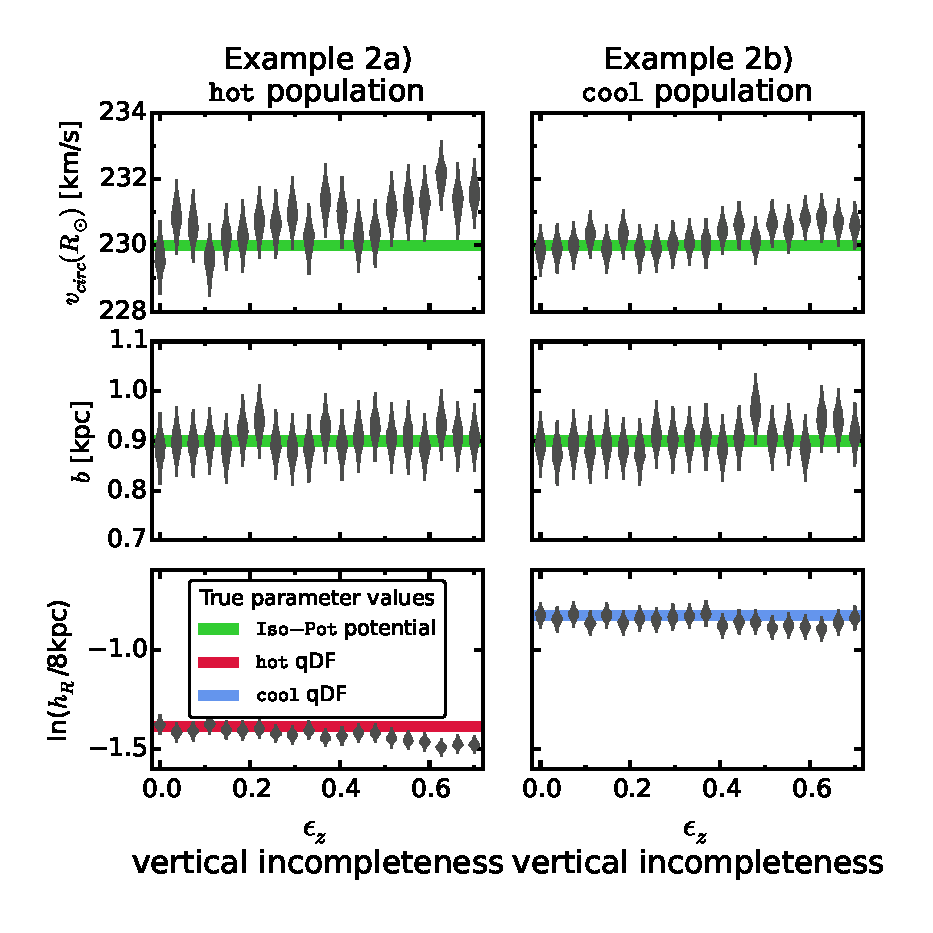
\includegraphics[width=0.8\textwidth]{figs/isoSphFlexIncompZ_violins_2.eps}
\caption{Influence of wrong assumptions about the incompleteness parallel to the Galactic plane of the data on the parameter reocovery with \RM{}. Each mock data set was created having different incompleteness parameters $\epsilon_z$ (shown on the $x$-axis and illustrated in Figure \ref{fig:isoSphFlexIncompZ_mockdata}) and the model parameters are given as Test \ref{test:isoSphFlexIncomp}, Example 2, in Table \ref{tbl:tests}. The analysis however didn't know about the incompleteness and assumed that all data sets had constant completeness within the survey volume ($\epsilon_z = 0$). The marginalized likelihoods from the fits are shown as violins. The green lines mark the true potential parameters (\texttt{Iso-Pot}) and the red and blue lines the true qDF parameters (\texttt{hot} \MAP{} in red and \texttt{cool} \MAP{} in blue), which we tried to recover. The \RM{} method seems to be robust against small to intermediate deviations between the true and the assumed vertical data incompleteness, as well as the radial incompleteness in Figure \ref{fig:isoSphFlexIncompZ_violins}.} 
\label{fig:isoSphFlexIncompZ_violins}
\end{minipage}
\end{figure}


\begin{figure*}
\plotone{figs/isoSphFlexIncomp_marginal_violins_2.eps}
\caption{Influence of wrong assumptions about radial and vertical incompleteness on the parameter recovery, when \emph{not} including information about the tangential velocities in the analysis. The mock data sets are the same as in Figure \ref{fig:isoSphFlexIncompR_violins} and \ref{fig:isoSphFlexIncompZ_violins}, but this time we did not include the data coordinates $v_T$ in the analysis and therefore marginalized the likelihood over $v_T$ instead (see \S\ref{sec:incompZ}). This demonstrates that much of the information about the potential is actually stored in the rotation curve, i.e. $v_T(R)$, which is not affected by removing stars from the data set. But even if we do not include $v_T$ we can still recover the potential within the errors, at least for small ($\epsilon_z \lesssim 10\%$).} 
\label{fig:isoSphFlexIncomp_marginal_violins}
\end{figure*}

\Wilma{[TO DO: Mention in text or caption how the panels looked that I removed.]}
